This chapter presents the context of our work. We will start with an overview of
the architecture of a modern HPC cluster, and then showcase several benchmarks
commonly used in HPC, which we will refer to later in this thesis (in the
context of the validation of our simulator).

\section{HPC clusters' architecture}

Our work focuses on the network aspect of High Performance Computing. We will
start with some context regarding HPC clusters, and then focus on the challenges
that interconnection network face, both at the hardware and software level.

\subsection{General overview}

Because of the physical limitations that CPUs face, High Performance Computing
(HPC) clusters use very specific hardware to get the most computing power
possible from each machine that composes the cluster, and they also have an
increasing number of machines connected together. This means that a typical
machine (referred to as ``node'' in this document) is usually composed not only
of one or more CPUs, but also one or more Network Interface Controller (NIC) and
possibly one or more accelerator for fast parallel computation. These nodes are
interconnected using switches of low-latency and usually high radix (i.e. a large
number of ports allows connecting many nodes or other switches), which enables
various topologies to be used. For example
Figure~\ref{fig:2_context_hpc:FatTree} depicts a simple fat-tree, with wider
links (higher bandwidth) closer to the ``root'' of the tree. On this example, we
can see that the distance between two nodes is variable: two machines connected
to the same switch will be able to communicate by traversing only two cables and
one switch, whereas nodes on opposite sides of the tree will need to traverse
four links and three switches to communicate, increasing the latency of network
transfers.

\begin{figure}[!ht]
    \centering
    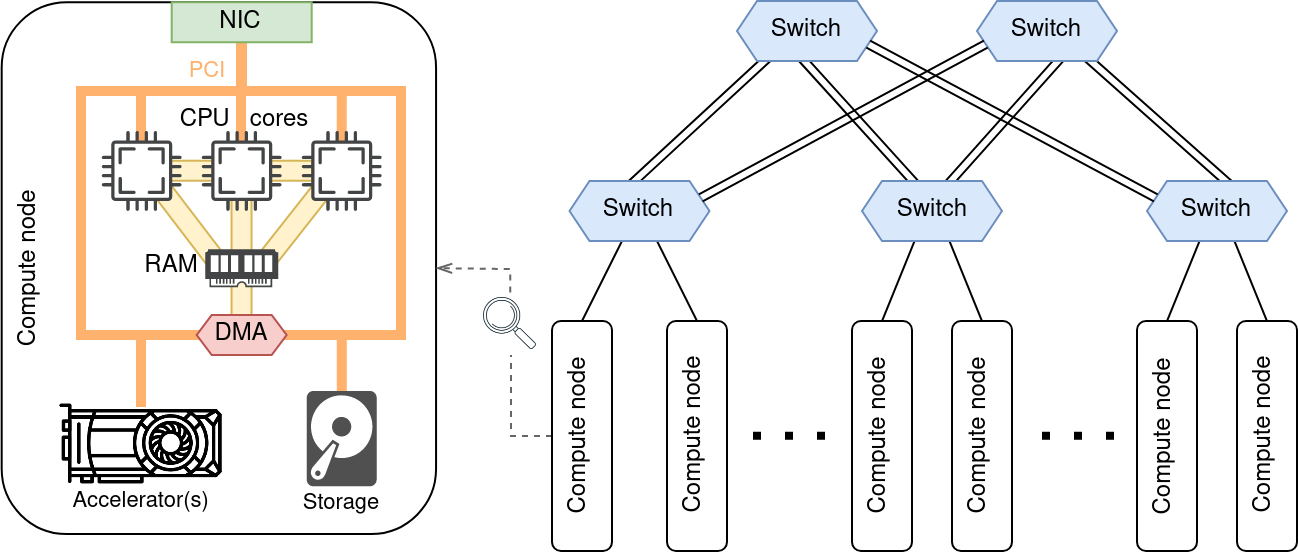
\includegraphics[width=1\textwidth]{2_context_hpc/fat_tree.png}
    \caption{Simplified cluster representation, with a zoom on a compute node}
    \label{fig:2_context_hpc:FatTree}
\end{figure}

While the diversity of hardware and increasing number of nodes makes clusters
more performant, it also makes it more difficult to predict the performance of a
cluster executing a given application, because of complex interactions between
each type of hardware on each node. A second side effect is that clusters become
increasingly more costly to build and run, which makes real-world experiments
very costly. The increase of the number of nodes also makes the topology of the
cluster more and more important: routers and cables are an expensive part of the
cluster, but it is crucial that they have a good performance, so connecting all
this hardware efficiently is very important. On
Figure~\ref{fig:2_context_hpc:FatTree} we can see that while nodes are usually
very similar to each other (a typical cluster will have many identical compute
nodes, and a few service nodes for login, storage, management, etc.), the
allocation of tasks on the cluster still matters, because of communications:
nodes that are on different switches will have to go through more links and
switches in order to exchange data, whereas nodes on the same switch will
benefit from a very low latency. We can also see that messages can take several
paths through the network when going from one node to another, which makes
efficient routing important.

There has been many studies in the field of interconnection networks and routing
algorithms, from which many topologies have emerged. To cite only the most
commonly used, the Flattened Butterfly~\cite{Kim2007} focuses on
cost-efficiency, by relying on path diversity, which shows the best result when
the routing algorithm used leverages adaptive routing, which means that switches
can decide which path to choose on a message-per-message or packet-per-packet
basis, instead of having a strict static route for each source-destination pair
(which improves the load-balancing abilities of the network).
Dragonfly~\cite{Kim2008} networks operate on the same idea, but they use groups
of switches to emulate a ``virtual router'' of even higher radix than the
underlying switches, which further reduces the cost of building the network,
while still showing good performance. Torus~\cite{Ajima2009} topologies are more
original since they do not use a traditional architecture with NICs on compute
nodes and switches to connect them together: instead every node has an
``interconnect controller'', which acts both as a NIC (with several
``communication engines'' to communicate with CPUs) and a small switch (with a
dozen of ports typically). This allows nodes to be connected in small groups,
and groups to be connected together along a variable number of dimension (up to
6D for the Tofu interconnect for example). Finally, the most common topology is
probably the Fat-Tree~\cite{Leiserson1985}, which has been extensively studied,
in order to improve routing~\cite{Gomez2007}, make accurate
simulations~\cite{Liu2015}, etc. It relies on a hierarchy of switches, with
compute nodes connected at the lowest level, and cables of increasing bandwidth
as we get closer to the root of the tree, as depicted earlier in
Figure~\ref{fig:2_context_hpc:FatTree}. Several routing algorithms have been
proposed on this topology, which rely on either static or adaptive
routing~\cite{Gomez2007}, and which try to balance the load as well as possible
between the different paths that are available in the tree. The most common is
D-Mod-K~\cite{Zahavi2010} but others exist, such as node-type-based
load-balancing~\cite{Gliksberg2018} which was proposed by Atos.

While our work could theoretically be used to study different topologies and
compare their performance, it will not be discussed in  detail in this thesis
because the interconnect that we work on, BXI, is mostly used with Fat-Trees in
production, therefore all our experiments will use this topology.

\subsection{Networking hardware}

In the world of High Performance Computing, there are several competitors when
it comes to production interconnection networks: the most notable are Cray
(acquired by HPE during this PhD), Mellanox (acquired by Nvidia during this
PhD), Fujitsu and Atos. Another noteworthy interconnection network is OmniPath:
while it has first been discontinued by Intel, it has since been bought by
Cornelis Networks, and there are several interesting studies on its performance
and modeling~\cite{Rosales2017}.

Cray's interconnects support a wide range of topologies: from Dragonfly network
in their latest Slingshot interconnect, to 3D-Torus in the Seastar
interconnect~\cite{Brightwell2005}. Torus networks have been shown to work in
higher dimensions, for example in 6D with the Tofu interconnect~\cite{Ajima2009}
made by Fujistu, which is used in the Fugaku supercomputer (number two on the
Top500 list as of the writing of this PhD). While early versions of Cray's
interconnect were known to use Portals 3 as their lower-level network API,
Slingshot is based on the Ethernet protocol~\cite{DeSensi2020}. On older
generations of interconnect (as the Gemini and Aries which are still used in
several clusters) the lowest software layer that is exposed to user code is
composed of two APIs: uGNI and DMAPP~\cite{Cray2010}. Cray's NICs typically
support bandwidths up to 200Gbits/s.

Mellanox's interconnects are the most popular option for new clusters. They
implement the standard Infiniband architecture~\cite{Pfister2001}, which is
supported by most (if not all) higher-level APIs. They also feature a variety of
hardware of different performance and price, such as the EDR and HDR series,
which explains their popularity for clusters of all sizes. At the
lowest level, users call the IB-verbs interface which is used to communicate
with the NIC. High-end NICs from Mellanox typically support bandwidths up to
200GBits/s, with the upcoming generation expected to support 400Gbits/s.

Atos's interconnect, BXI, will be our case study for this PhD. It implements in
hardware the Portals 4 network API, and is used in some of the fastest European
supercomputers. It is one of the youngest interconnect of the market, with NICs
supporting bandwidths up to 100Gbits/s, but it has showed very good results so
far, equipping supercomputers with a very good rank in the Top500 list:
Tera-1000-2 was at the 14\textsuperscript{th} place worldwide and n°1 in Europe
at the time of its installation~\cite{top500_tera1000}, and currently Exa1-HF
holds the 20\textsuperscript{th} place worldwide~\cite{Top500_exa1} (it was also
14\textsuperscript{th} at the time of its installation in 2021).

All these interconnects share a few similarities: their main goal is to offload
as much network processing from the CPU as possible. This is made possible using
a few properties that differ from traditional networking hardware: first,
OS-bypass allows user code to send commands to a NIC without any system call,
which speeds up communications significantly. Most NICs also provide zero-copy
processing, which implies that incoming messages can be processed fast enough so
that the incoming data is routed to the correct location in memory without being
copied in intermediate buffers. This is made possible either by pinning memory
pages used for network communications (as Mellanox's hardware does), or by
having a full Virtual-to-Physical (V2P) circuit on the NIC (as does Atos's BXI
hardware).

While the simulation of other interconnects and network APIs have been studied
in depth, for example the congestion on Infiniband networks
by~\cite{Vienne2010}\cite{Gran2012}, Intel OmniPath with
OpaSim~\cite{Javier2018}, or Cray's interconnect~\cite{Mubarak2017}, very few
studies have been conducted on BXI, and the existing ones focus on very specific
problems, such as the update of routing tables when the topology
changes~\cite{Vigneras2016}. In this thesis we will propose a model for Portals
4 and tune the simulator for accurate simulations of the BXI interconnect.

\subsection{Networking Software Stack}
\label{subsec:2_context_hpc:software_stack}

While the typical software stack for HPC communications is very different from
the traditional OSI layers, it features similar levels of abstraction (depicted
on Figure~\ref{fig:2_context_hpc:HpcSoftwareStack}). We will start by giving a
global overview of these layers, before presenting Portals in more details in
the next section, since it is the lowest-level software layer used at Atos, and
it will be the most important from the point of view of our
simulator.

\begin{figure}[!ht]
    \centering
    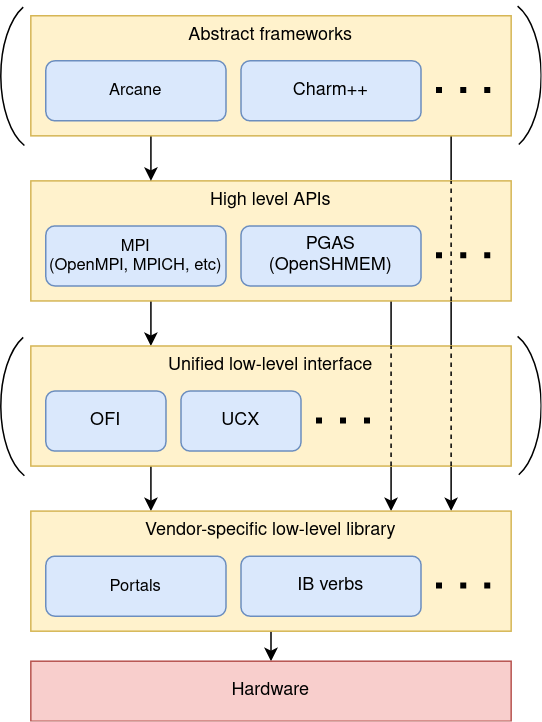
\includegraphics[width=0.6\textwidth]{2_context_hpc/HPC_software_stack.png}
    \caption{HPC software stack}
    \label{fig:2_context_hpc:HpcSoftwareStack}
\end{figure}

At the lowest level, there is usually a very thin software library (potentially
coupled with a kernel module), that directly interacts with the hardware, and
exposes a few primitives with a very low level of abstraction to user code. It
usually only performs point-to-point operations between two machines, and does
not have any notion of collective operations involving several machines. For
Infiniband this layer is called IB-verbs, and for Atos's BXI interconnect it is
the Portals 4 API directly, as it is fully implemented by the NIC in hardware.
It is this Portals 4 layer that our simulator will model, as it will provide a
model of the behavior of the NIC.

Above this layer, high-level APIs provide more abstract features that allow
programmers to write efficient code, focusing on the algorithmic aspects and
abstracting away the implementation details of communications. In this category,
several programming models exist: for example Partitioned global address space
(PGAS), with implementations such as OpenSHMEM~\cite{Chapman2010}, allow user
code to have a transparent representation of memory that is distributed on
several machines. The most popular of these programming models is without a
doubt the Message Passing Interface (MPI)~\cite{Graham2006}, which offers many
ways of communicating: onesided, where a target machine exposes memory regions
that other machines can query ; regular point-to-point operations where both
machines are actively involved (using send and receive primitives) ; and finally
collective operations which provide abstract communication primitives such as
all-to-all pattern, gather (N to 1 communication), scatter (1 to N), and even
simple data processing with reduce, allreduce, etc. primitives. These collective
operations usually have several implementations, which can be chosen dynamically
depending on the message sizes and the number of machines involved in the
operation. There are many MPI implementations, such as OpenMPI, MPICH, IntelMPI,
etc. We will study OpenMPI in particular, as it is the MPI implementation that
is officially supported by our case study interconnect, BXI. It is worth noting
that our version of OpenMPI is a fork optimized by Atos for BXI, which we will
explain in more detail in Chapter~\ref{chap:high_level}. These high-level APIs
are sometimes criticized for their cost in terms of performance, in particular
MPI~\cite{Raffenetti2017}, but their compromise between ease of use and
performance makes them the standard to write HPC applications. Some projects
even try to replicate this type of programming model in hardware,
as~\cite{DeMatteis2019} does on Field Programmable Gate Arrays
(FPGAs).

These two layers are the most important and will usually exist in any HPC
software stack, but there can also be additional ones: in particular some APIs
try to provide a unified interface between the low-level transport and the
high-level abstract API. The goal of this added layer is to limit the number of
implementations that need to be made in high-level APIs to accommodate for any
possible low-level transport. This is similar to the intermediate representation
compilers use, which allows them to have only $N$ frontends and $M$ backends to
be able to compile $N$ languages into $M$ machine codes, instead of having $N
\times M$ complete toolchains. These interfaces include the Open Fabric
Interface (OFI)~\cite{Grun}, of which Atos made an implementation built with
Portals (in order to support BXI), as well as Unified Communication X
(UCX)~\cite{Shamis2015} or Nemesis~\cite{Pritchard2011} for example.

Finally, while high-level APIs are already more user-friendly than low-level
transports, they are still very general purpose and offer much control, which is
why some frameworks can be used on top of them for even more abstraction. They
can be domain-specific, as Arcane~\cite{Grospellier2009} for example, which is a
tool made by the CEA to build physics simulators on top of MPI. Some libraries
like SkePU~\cite{Enmyren2010} provide complete data-processing algorithms on
distributed data, for example MapReduce, Stencils, etc. Some frameworks expose a
unified API to execute algorithms on heterogeneous architectures (for example by
exploiting local parallelism with OpenMP\footnote{OpenMP is an API for parallel
processing across CPU cores, which relies on compiler directives and a library},
inter-machine parallelism with MPI, etc.) like StarPU~\cite{Augonnet2011}. Some
approaches even go as far as designing a full programming language for parallel
processing, such as Chapel~\cite{Parenteau2021}, which implements a PGAS model
and uses low-level transports directly, or Charm++~\cite{Kale1993}, which
provides automated load balancing and supports MPI as its transport mechanism.

\begin{figure}[!ht]
    \centering
    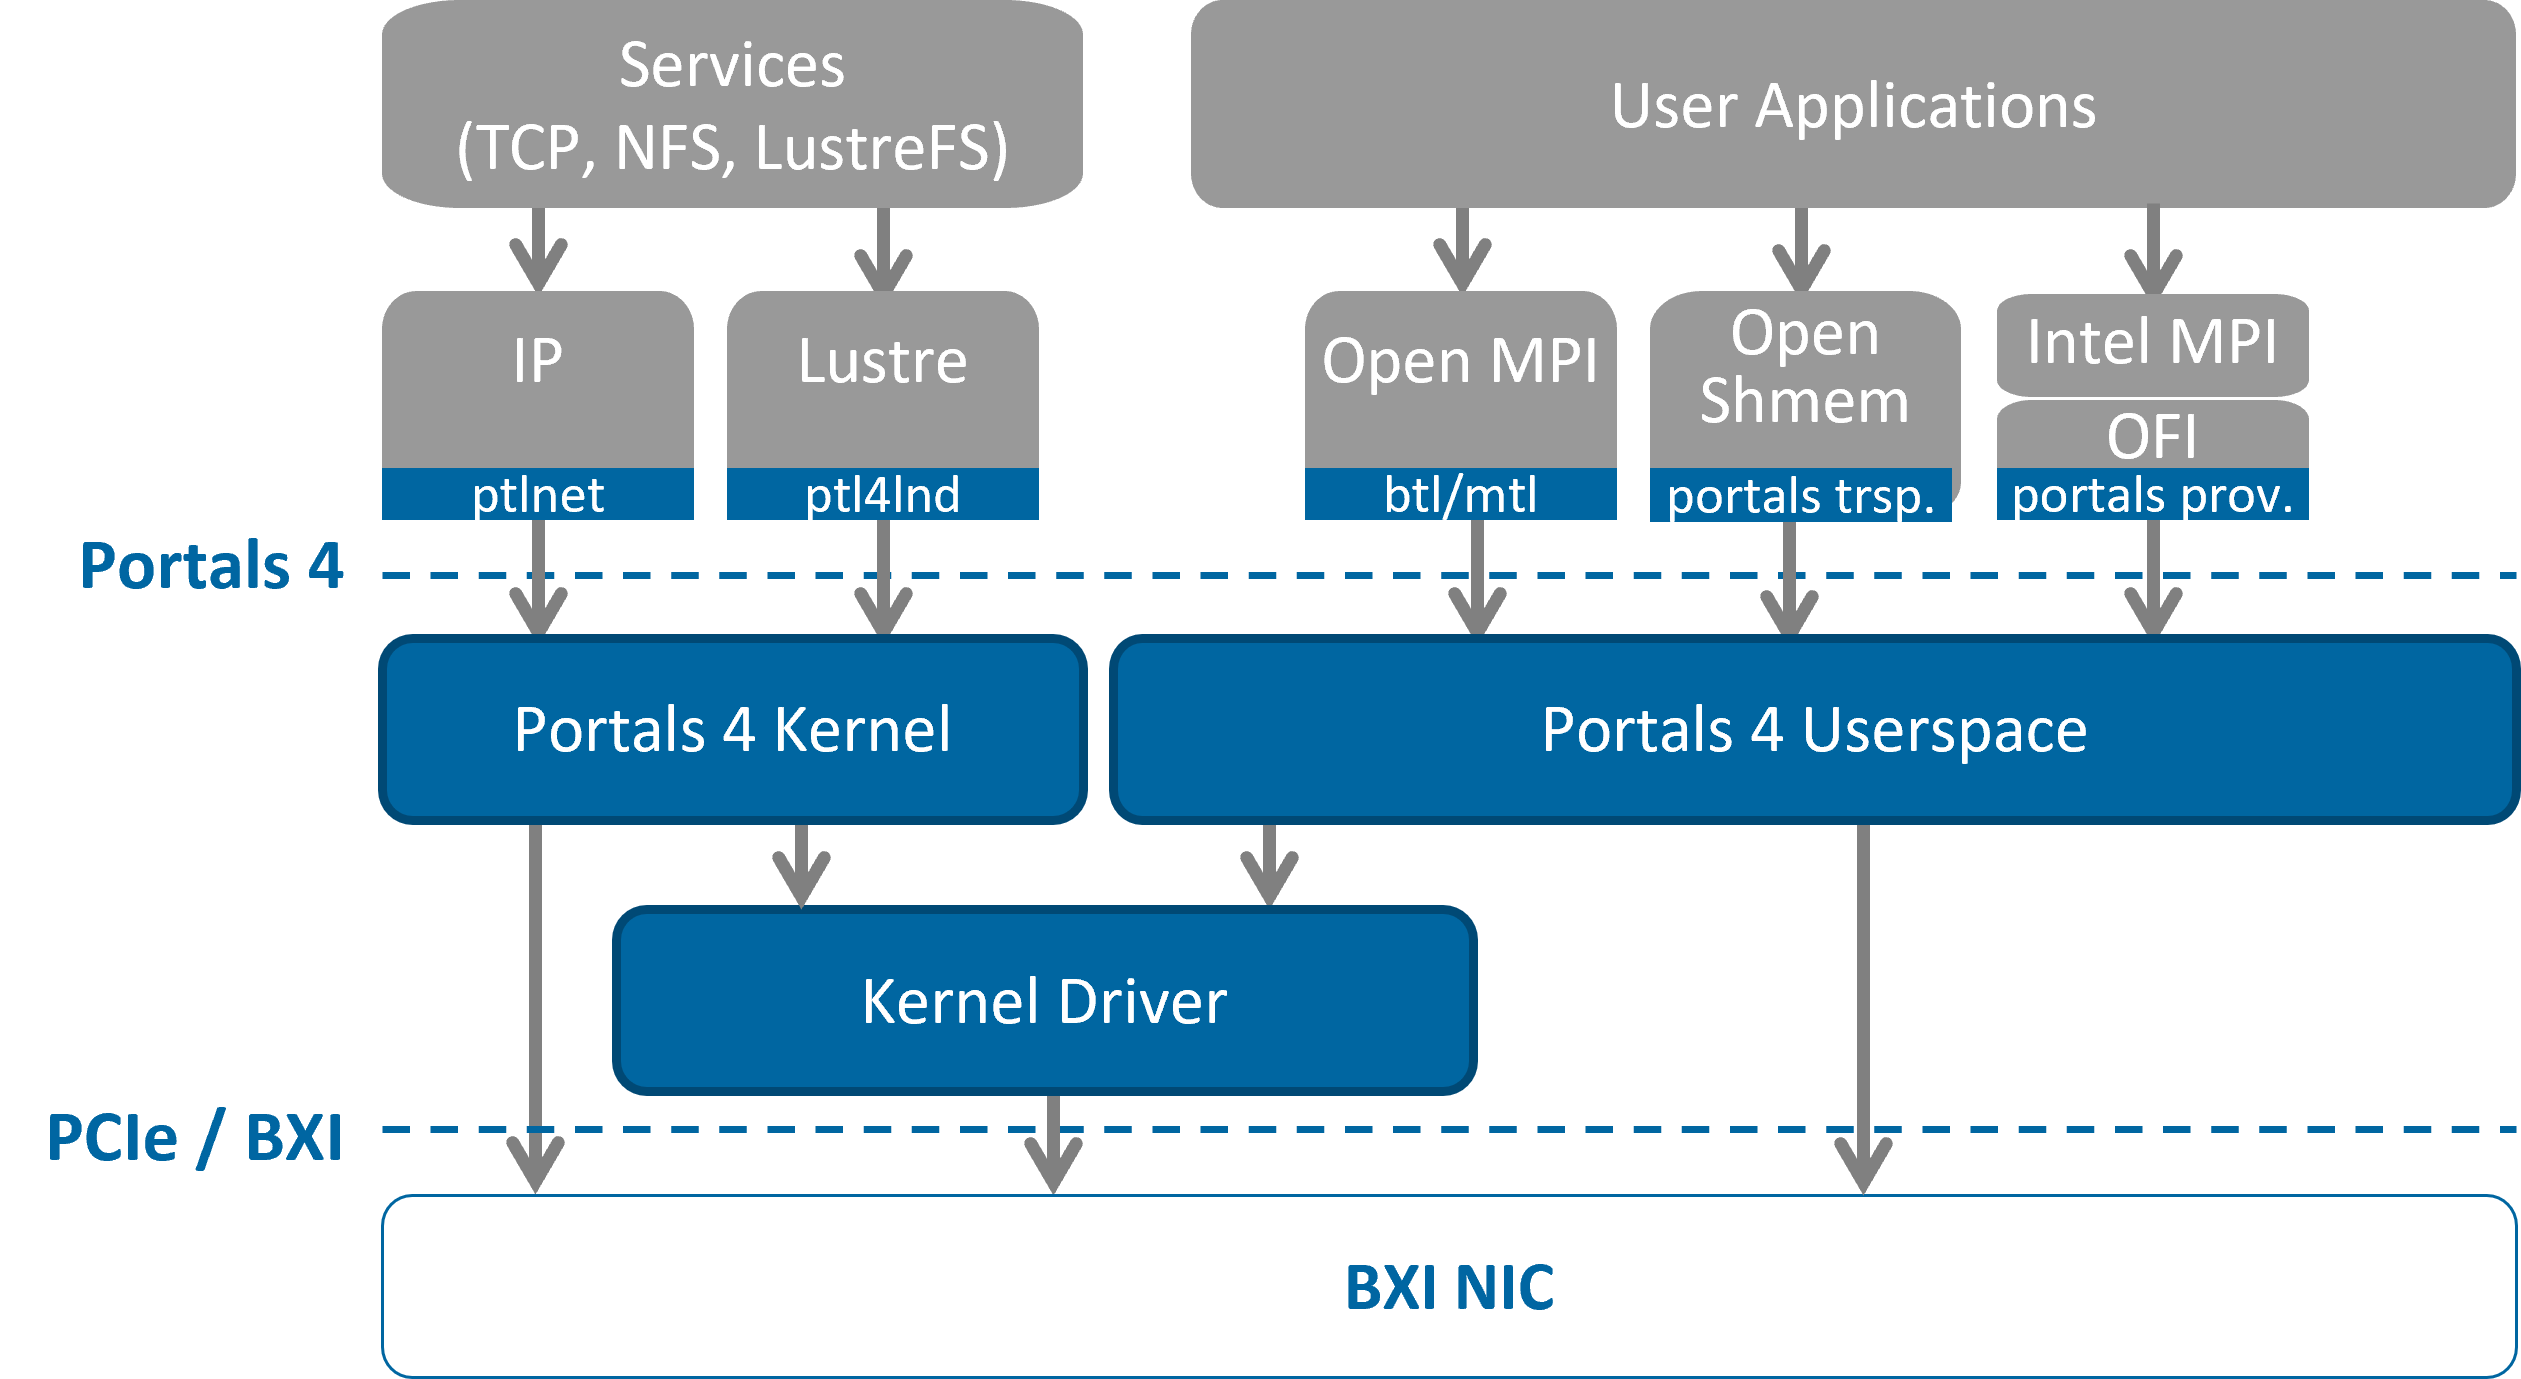
\includegraphics[width=0.9\textwidth]{2_context_hpc/atos_stack.png}
    \caption{Atos's software stack on top of BXI NICs}
    \label{fig:2_context_hpc:AtosSoftwareStack}
\end{figure}

The software stack used at Atos, which is going to serve as a case study for
this thesis, is depicted on Figure~\ref{fig:2_context_hpc:AtosSoftwareStack}. It
is based on Portals, which we will describe in more detail in the next section,
and supports a wide range of higher level APIs and services: it can emulate the
Ethernet protocol using a layer called Ptlnet, supports the Lustre distributed
Filesystem, provides different APIs for fast computation such as OpenMPI,
OpenSHMEM, and IntelMPI (on top of OFI), etc. In this thesis we will study in
detail OpenMPI in particular, and we will discuss OpenSHMEM support.

\section{The Portals API}

Portals is a standard HPC API specified by Sandia National
Laboratories~\cite{Brightwell2022}. It has been used in supercomputers for
decades, with a few success stories like the ASCI Red
supercomputer~\cite{Mattson1998}, which was the first to break the Teraflop
barrier in 1996 using an early version of Portals. Since then Portals has been
used mainly by Cray, and nowadays its main implementation is in the BXI
interconnect made by Atos. This API provides connectionless, reliable
communications using Remote Direct Memory Accesses (RDMA). While many details
about the underlying protocol are left to the implementation, Portals is
designed with OS-bypass in mind, and it should enable a ``natural''
implementation of MPI two-sided primitives, as well as PGAS one-sided
operations.

\subsection{Portals data structures}

Portals features several data structures to interact with the hardware, which
are defined in the Portals's specification~\cite{Brightwell2022}. This section
presents the most important ones in the context of our work.

\subsubsection{General purpose structures}

\portalsAbbr{Network Interfaces}{NI} act as an ``entry'' point, which represents
the interface with the hardware. In Portals the addressing is analogue to IP
addressing, since each physical NIC has a \portalsAbbr{Node Identifier}{NID},
which is the equivalent of IP addresses (although it is a simple number instead
of a full address), and each NI (which usually corresponds to a single
application process) has a unique \portalsAbbr{Process Identifier}{PID}. In
those NIs, one or more \portalsAbbr{Portal Table}{PT} stores the data structures
that will be used for the reception of messages. The pair $\{PID ; PT\}$ is
similar to ports in an IP-based stack.

\subsubsection{Reception data structure}

\portalsAbbr{Matching Entries}{ME} are used to configure the reception of
incoming messages. A matching entry stores the address and length of the memory
space where incoming messages' data should be written, as well as match bits and
ignore bits. Match bits are a set of 64 bits which allows an efficient routing
of data at the receiver side: when an initiator sends a request, it includes
match bits in the message, and the target uses these bits to identify which ME
should be used to process the request, by testing each ME against the incoming
message using the following criterion:

\begin{center}
    $((incoming\_bits \; \wedge \; match\_bits) \;\;\; \& \;\; \sim\!ignore\_bits) \: == \: 0$
\end{center}

\begin{figure}[!ht]
    \centering
    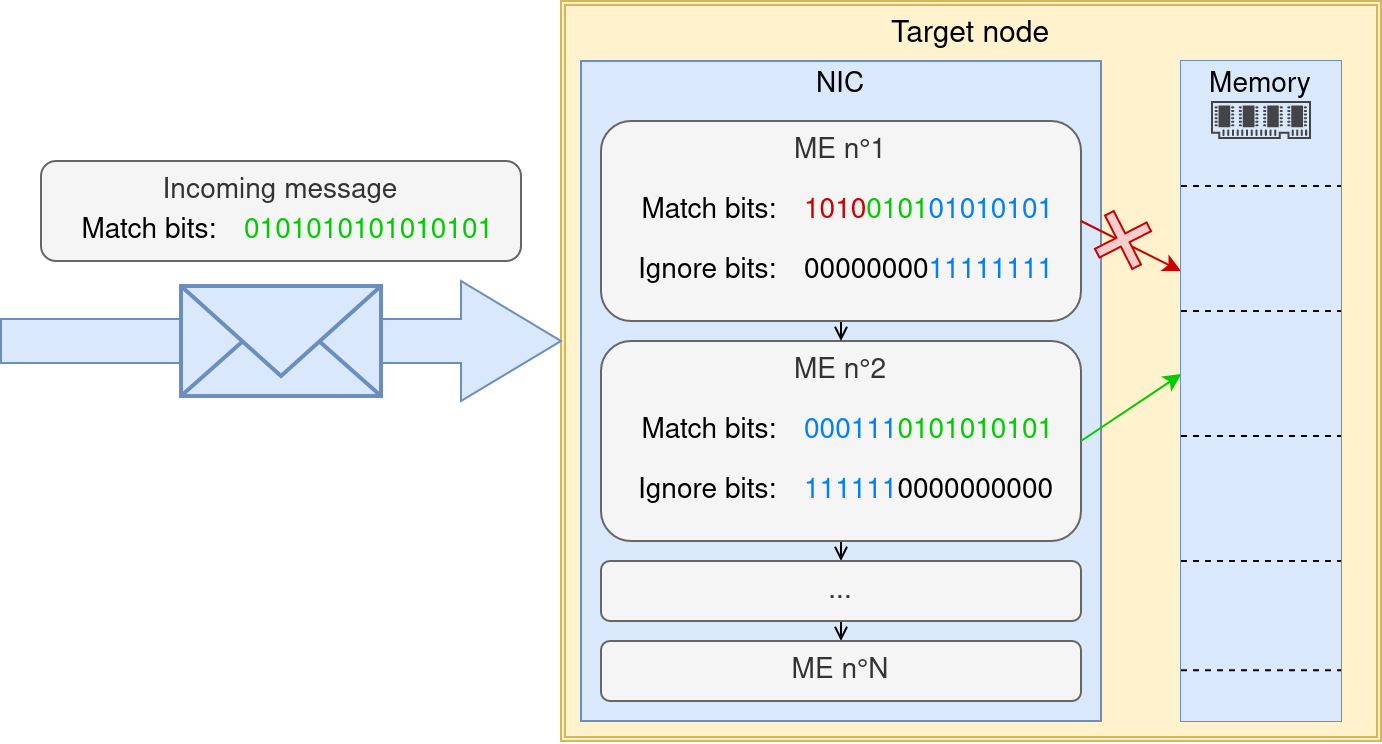
\includegraphics[width=1\textwidth]{2_context_hpc/match_bits.png}
    \caption{Example of matching between MEs and an incoming request}
    \label{fig:2_context_hpc:matching}
\end{figure}

The first ME to match the incoming request is then used to determine on which
memory region the requested operation needs to be performed. An example is shown
on Figure~\ref{fig:2_context_hpc:matching}, where we can see that nodes can have
several MEs, which map to different locations in memory. To determine which ME
needs to be used when processing an incoming request, Portals loops through the
available MEs, and looks at match bits, using the opposite of the ignore bits as
a mask (so the only match bits that are relevant are the positions where there
is a 0 in the ignore bits). If those bits are the same as in the incoming
message, the ME is used to process the message (in order to determine the memory
location where the incoming payload should be written). In the example, the
first ME does not match, because the first bits are not ignored and they are
different from the first bits of the incoming message, whereas the second ME
matches because even though the first bits are different, they are ignored, and
all the ending bits are identical to the bits of the incoming message.
Therefore, the payload from the incoming message is stored in the memory
location referenced by ME n°2.

MEs feature a variety of options that affect their behavior: they can have one
or several uses, as well as locally manage the offset at which messages are
written after each operation (by default this offset is specified on the sender
side), etc. Portals also features more simple \portalsAbbr{List Entries}{LE},
which function exactly as MEs, but do not use match bits or ignore bits, which
means that every incoming message will match the first LE posted in the Portal
Table.

\subsubsection{Transmission data structures}

The data structure for transmission is more simple than the structures for
reception: \portalsAbbr{Memory Descriptors}{MD} are simply used to represent the
start and length of the memory zone that needs to be sent on the network. They
also feature a few options, but which do not change drastically their behavior:
these options mostly impact which events need to be emitted or not.

\subsubsection{Event systems}

Portals feature two distinct event systems, which allow users to be notified of
the activity on the network by attaching data structures to a PT, an MD or an
ME.

The first, more complete system involves \portalsAbbr{Event Queues}{EQ}, which
record full events with detailed information on the corresponding operation,
such as the type of event, an error code, and a variable number of fields
depending on the type of the event (for example the NID of the remote peer who
caused the event, or the amount of data that was impacted, etc.). EQs can be
associated with PTs and MDs.

The second system is more lightweight: instead of EQs, it uses
\portalsAbbr{Counting Events}{CT}, which do not record any information about the
operations that is in progress. Instead, each CT features two counters that
track successful operations and failed operations. CTs can either count by
incrementing by one each time, or incrementing by the number of bytes that was
manipulated in the corresponding operation (based on a flag at their creation).
CTs can be associated with MEs and MDs.

Both systems can be queried through a variety of function, which can search for
events (or a certain value in CTs) in a way that is either asynchronous or
blocking, while looking at either one or several EQ/CT.\newline

\subsection{Communication primitives}

Portals features several operation types to exchange and manipulate data. All
these operations are strictly point-to-point, as Portals does not have a concept
of collective operation.

\subsubsection{PtlPut}

Put operations are a very basic ``send'' operation, which corresponds to an RDMA
write. As most operations, it can have match bits or not, and it will trigger
various events that users can listen to: in particular a ``SEND'' event when the
user buffer (which contains the data to be sent) can be safely re-used and an
``ACK'' event when an acknowledgement has been received from the remote node
that was targeted. At the target, Put operations trigger a ``PUT'' event.

\subsubsection{PtlGet}

Get operations correspond to an RDMA read: making a Get request only sends a
small message to ask the remote machine for a piece of memory, at which point
the remote NIC will send back the requested data in a response. Unlike Put
operations this means that the request is very lightweight (only a few bytes of
metadata) and the payload which can have an arbitrary size is in the response
instead. From a user perspective, the completion of the operation can be tracked
by listening to a ``REPLY'' event. At the target, Get operations trigger a
``GET'' event.

\subsubsection{PtlAtomic}

Atomic operations operate in a way that is very similar to a Put, but the NIC
also performs an arithmetic operation using two operands: the incoming payload
and the data already present at the specified address in the remote node's
memory (which is also used to store the result). These operations can be a sum,
product, etc. on various data types (integers, floating point numbers, etc.).

\subsubsection{PtlFetchAtomic}

FetchAtomic operations work in the same way as Atomics, but they also send a
full response which contains the piece of data before it was modified by the
Atomic operation. This means that FetchAtomic behaves as an Atomic and a Get at
the same time: the request contains data to be used by the Atomic operation, but
the response also contains data to be written at the initiator side as in a
traditional Get. This also means that the operation involves two MDs at
initiator side: one to describe the data to be sent and one to store the
incoming response.

This operation has a variant, called PtlSwap, which operates very similarly to
\inline{PtlFetchAtomic} except that the permitted operation types are not
arithmetic operations but different variations of swaps (conditional, with a
mask, etc.).


\subsection{Portals's implementation in BXI}

While Portals is a good specification for the API that should be exposed to
users, at the lowest level significant freedom is left to the implementation. In
this section we will present a few properties of BXI's implementation of Portals
which will be of interest when modeling Portals in our simulator.

\subsubsection{End-to-End (E2E) Reliability}
\label{subsubsec:2_context_hpc:E2E}

Since Portals is a reliable network API, it is the responsibility of BXI NICs to
ensure that messages are delivered without errors. At packet-level the integrity
of the data is enforced using a Cyclic Redundancy Check (CRC): each network
packet features a field in its header for CRC data, which allows the receiver of
messages to check the integrity of the payload, and send an acknowledgement
(ACK) with an error code if any packet was corrupted, which will trigger a
retransmission of the message by the sender. At message-level, a system of
timeouts and retries is implemented using a dedicated ``E2E'' circuit. This part
of the NIC keeps track of all outgoing messages, and if no acknowledgement is
received within a configurable delay, the NIC will retransmit it. This happens a
tunable number of times until the message is eventually given up on. An
interesting property to note is that since ACKs are important messages that need
to be reliably transmitted to ensure all events are properly generated, BXI
implements two levels of ACKs. We will call ``Portals ACK'' the messages that
acknowledge the reception of a Put or Atomic operation (which can cause the
emission of an ACK event for the user application), and ``BXI ACK'' the messages
that acknowledge the reception of a Portals ACK (which is only used internally
by the E2E logic to know that a Portals ACK message does not need to be
retransmitted, in a way that is entirely transparent to the user application).

\subsubsection{Virtual Networks (VN)}
\label{subsubsec:2_context_hpc:VNs}

According to the Portals specification, it is required for messages to be
ordered. This means that commands issued to the NIC by the user should result in
messages being sent on the network in the same order, and also that this order
should match the order of receptions at the target (in case all messages target
the same machine). This causes a practical issue in real-world scenarios, which
can lead to a complete deadlock of a NIC in the worst case: for example if
fetching the data that needs to be sent by a request triggers a page fault which
can only be resolved with another Portals request (if this data is located on a
Network File System for example). Such dependencies between requests are solved
by allowing different VNs to progress independently: BXI supports a total of
four VNs: a ``COMPUTE'' VN for requests, a ``COMPUTE'' VN for responses, a
``SERVICE'' VN for requests and a ``SERVICE'' VN for responses. In our previous
example, the problem would be solved by starting the NFS in ``SERVICE'' mode
while having the main application in ``COMPUTE'' mode.

This system also allows requests and responses to progress independently: for
example a small ACK can progress even if a large request is in progress. This last
property is to be taken with a grain of salt: even though the vast majority of
the processing in the NIC allows all four VNs to progress independently, at the
very end (writing the packets physically on the network cable) messages are once
again sequential, and packets from different messages cannot be
interleaved.

\section{Benchmarks of interest}
\label{sec:2_context_hpc:benchmarks}

In HPC, there is a wide variety of benchmarks that are used to assess the
performance of a cluster. The diversity of these applications comes from the
need to evaluate performance at different scales, for example with low-level
utilities to evaluate the speed of communications between a pair of machines, or
at the opposite full scale applications which exhibit more complex behavior but
which are also a more realistic use-case of an HPC cluster. Benchmarks can also
have different goals in terms of workload: some are more network-intensive,
others will focus on CPU usage, etc. The original use-case of most benchmarks is
to evaluate the performance of real clusters. In contrast, this thesis focuses
on simulation, and we will use the same benchmarks to assess the accuracy of our
models. We will therefore run these benchmarks both on real-life clusters and in
simulation to compare the results.

Additionally, the applications in which execution flow does not depend on the
manipulated data can be adapted in skeleton versions, where the execution flow
and communication patterns are preserved but most of the expensive computation
phases are removed. Skeleton versions of applications are especially useful to
study the network's performance, in particular in simulation where the
computational phases can be replaced by an increase of the simulated time, as we
will see in more detail in Chapter~\ref{chap:high_level}.

This section will present the benchmarks we chose to use in this thesis, from
the most simplistic low-level utilities to the most complete applications.

\subsection{Network benchmarks}

\subsubsection{Ptlperf}
\label{subsubsec:2_context_hpc:ptlperf}

Ptlperf (short for ``\textbf{P}or\textbf{t}a\textbf{l}s \textbf{perf}ormance'')
is a tool developed at Atos, whose goal is to measure the network speed between
two NICs using the Portals 4 API. It has various modes, which replicate more or
less realistic scenarios:
\begin{itemize}
    \item Fast mode sends as many messages on the network as possible without
    caring for acknowledgements or any other Portals event. It makes the
    resulting workload unrealistic, but it showcases the theoretical maximum
    transmission speed of the hardware.
    \item ACK mode counts completed requests by keeping track of
    acknowledgements from the target, a new message is sent each time the ACK
    event from the previous request is received.
    \item CT mode works in similarly, but it uses lightweight counters instead
    of full events to keep track of completed transfers, sending one message at
    a time.
    \item Reply mode implements a ping-pong instead of sending messages in one
    direction only.
    \item Match mode mimics a more realistic use case with several messages
    inflight, and a more realistic use of resources at the target side (MEs).
\end{itemize}

\subsubsection{OSU Micro Benchmarks}

Ohio State University (OSU) benchmarks are a set of dozens of ``unit test''
style benchmarks, made by the creators of the MPI implementation MVAPICH,
targeted at MPI and OpenSHMEM: each benchmark calls a specific primitive in a
short warm up loop and then a measurement loop, in order to determine its
performance on increasingly large messages. While this creates highly artificial
workloads, that do not correspond to a real-life scenario, it is an efficient
and standard way to measure the performance of a specific primitive in a
cluster. In essence, they are similar to Ptlperf in that they benchmark a
specific primitive, even though the methodology is slightly different, since OSU
benchmarks time a fixed number of calls, whereas Ptlperf tries to fit as many
calls as possible in a fixed amount of time.

\subsection{Realistic (proxy) applications}

While low-level network benchmarks are a good entry point to evaluate the
performance of an interconnection network, or the accuracy of a network
simulator, they do not represent realistic workloads. Using more realistic
applications is then important to evaluate the interactions between network
operations, computations, I/O operations, etc., and we will use the following
ones in our study.

\subsubsection{LULESH}
\label{subsubsec:2_context_hpc:LULESH}

\begin{figure}[!ht]
    \centering
    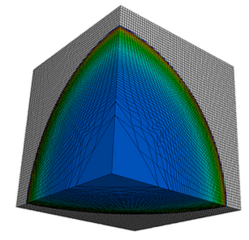
\includegraphics[width=0.4\textwidth]{2_context_hpc/LULESH.png}
    \caption[Visual representation of LULESH results]{Visual representation of LULESH results\protect\footnotemark}
    \label{fig:2_context_hpc:LULESH}
\end{figure}

\footnotetext{Image from \url{https://asc.llnl.gov/codes/proxy-apps/lulesh}}

Livermore Unstructured Lagrangian Explicit Shock Hydrodynamics (LULESH) is a
very popular C++ proxy application that is commonly used to benchmark HPC
clusters~\cite{Karlin2013}. The underlying physics problem that it solves is a
specific instance of a hydrodynamics problem, more specifically a Sedov blast
wave problem, which studies the deformation of materials in 3D, as explained
in~\cite{Hornung2011}. A graphical representation of an example result is
displayed on Figure~\ref{fig:2_context_hpc:LULESH}. As this application is very
popular, implementations of LULESH exist for most parallel programming
frameworks and hardware.

LULESH mainly uses point-to-point operations for its communications, along with
more occasional Reduce and AllReduce calls. The execution flow of the
application depends on the numerical results from computation, which is why it
is difficult (if at all possible) to make a skeleton version of this
application. It also has a constraint on the number of processes that need to be
used to run it: because of the way work is distributed on the MPI ranks, the
total number of process must be the cube of an integer (so 1, 8, 27 are valid
numbers of ranks for example).

\subsubsection{Quicksilver}

\begin{figure}[!ht]
    \centering
    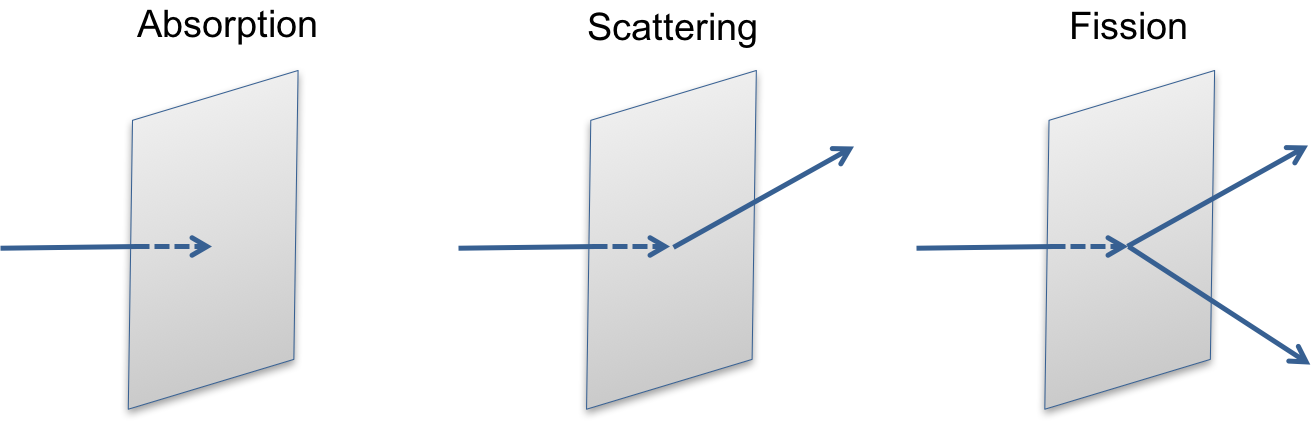
\includegraphics[width=0.6\textwidth]{2_context_hpc/Quicksilver.png}
    \caption[3 possible interactions that a particle can have in the Quicksilver model]{3 possible interactions that a particle can have in the Quicksilver model\protect\footnotemark}
    \label{fig:2_context_hpc:Quicksilver}
\end{figure}

\footnotetext{Image from \url{https://asc.llnl.gov/codes/proxy-apps/quicksilver}}

Quicksilver is a C++ proxy application that uses a Monte Carlo
algorithm~\cite{Carter1975} to solve a particle transport problem: it models a
configurable number of particles, and their interactions in 3 dimensions with a
predefined mesh. The possible interaction types are represented on
Figure~\ref{fig:2_context_hpc:Quicksilver}. Quicksilver has implementations both
on CPU, with OpenMP and MPI, and on GPU with CUDA.

It features a variety of point-to-point and collective operations, as well as
custom datatypes, which makes it an interesting app to study. However, similarly
to LULESH it is very hard to make a skeleton version for it as execution flow
depends on the correctness of calculations.

\subsubsection{HPL}

\begin{figure}[!ht]
    \centering
    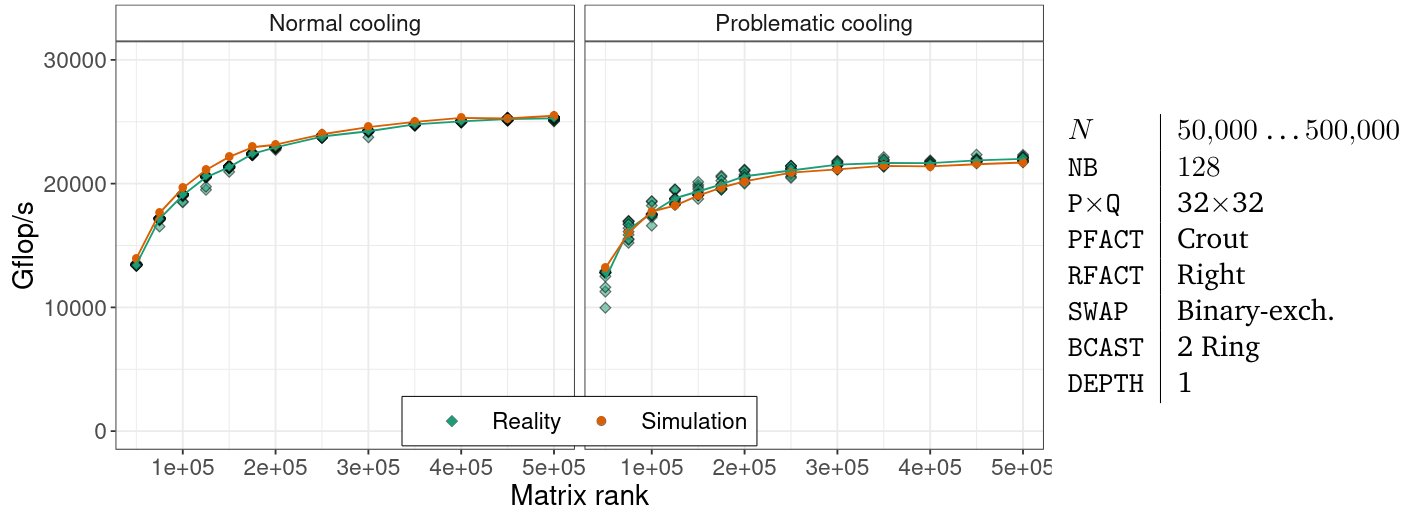
\includegraphics[width=1\textwidth]{2_context_hpc/HPL_Tom.png}
    \caption[Results of HPL simulation in SMPI in two scenarios]{Results of HPL
    simulation in SMPI in two scenarios. Image from~\cite{Cornebize2021}}
    \label{fig:2_context_hpc:HPL_Tom}
\end{figure}

High-Performance Linpack (HPL) is a very popular benchmark, famous for being
used to rank supercomputers in the Top500 list~\cite{Top500}. It solves a
mathematical problem, more specifically a randomly generated dense linear
system. The algorithm that is implemented is a lower-upper (LU) decomposition.

It relies on MPI for its communication, and on the Basic Linear Algebra
Subprograms (BLAS)~\cite{Lawson1979} for computation, which is a library that
has many implementations, some generic and some vendor specific. For example,
AMD provides its own version of BLIS~\cite{VanZee2015}, a framework that
provides a fast BLAS implementation, which is optimized for AMD CPUs (in
particular the Epyc and Ryzen architectures), and which is the version we will
use in our experiments.

HPL does not use any collective operation from MPI directly, instead the
application re-implements all collective primitives itself (using combinations
of point-to-point operations), and allows users to tune the algorithm used for
each type of operation in the input file that drives the execution.

What makes it an interesting application to study is that it has already been
the subject of many studies, and therefore it already has existing skeleton
versions: in this thesis we will be able to reuse a skeleton made for SMPI with
no modifications. Simulation results obtained with SMPI in two scenarios (with
or without a cooling incident on the cluster) are shown on
Figure~\ref{fig:2_context_hpc:HPL_Tom}. It also makes heavy use of user-made
datatypes and communicators (by splitting the global ``MPI\_COMM\_WORLD''),
which is not very common, so it is a good way to test these features in
simulation.
